\documentclass[12pt]{article}
\usepackage{setspace}
\linespread{1.2}
\usepackage{fullpage,graphicx,psfrag,amsmath,amsfonts,verbatim}
\usepackage[small,bf]{caption}
\usepackage{amsthm}
% \usepackage[hidelinks]{hyperref}
\usepackage{hyperref}
\usepackage{bbm} % for the indicator function to look good
\usepackage{color}
\usepackage{mathtools}
\usepackage{fancyhdr} % for the header
\usepackage{booktabs} % for regression table display (toprule, midrule, bottomrule)
\usepackage{adjustbox} % for regression table display
\usepackage{threeparttable} % to use table notes
\usepackage{natbib} % for bibliography
\usepackage{tikz}
\usepackage{subcaption} % for subfigures

\input newcommand.tex
% \renewcommand{\thesubsection}{} 
\bibliographystyle{apalike}
% \setlength{\parindent}{0pt} % remove the automatic indentation

\title{\small{\textbf{An Adversarial Approach to Structural Estimation}}}
\author{Tetsuya Kaji \and Elena Manresa \and Guillaume Pouliot}
\date{Presented by Zixuan, Huixin}

\begin{document}
\maketitle
% \thispagestyle{empty}
% \begin{abstract}

% \end{abstract}

% \newpage
% \thispagestyle{empty}
% \tableofcontents
% \newpage

% \setcounter{page}{1}

\section{Adversarial Framework} \label{sec:framework}

\citet{kaji2023adversarial} propose a simulation-based method of estimation. From my understanding, this method is a specific case of the more general Generative Adversarial Networks (GANs) framework, with the restriction that the data-generating process is characterized by a structural model. Since there are existing simulation-based methods such as Simulated Method of Moments (SMM) and Simulation Maximum Likelihood (SML), the paper contributes to this strand of literature by both making comparison of performance and deriving formal statistical results. To provide a thorough understanding of \citet{kaji2023adversarial}, we will first delve into a detailed explanation of the ideas underlying GANs.

\subsection{Mathematical Formulation} \label{subsec:math_formulation}
In this section, we lay out the basic mathematical framework of the adversarial
approach. While adversarial min-max zero-sum games are not new, their
implementation and adaptation in generative tasks—such as image generation—were
first proposed by \citet{goodfellow2014generative} and have been shown to
perform exceptionally well under various settings. By iteratively training a
discriminator that attempts to distinguish real data from fake data, and a
generator that responds by producing increasingly realistic synthetic data, the
algorithm can generate new objects that closely resemble existing ones. The
mathematical formulation of this game is as follows:
\begin{equation} \label{eq:gan_objective}
    \min_G \max_D L(D, G)
    = \mathbb{E}_{x_r \sim p_{r}(x)} [\log D(x_r)] + \mathbb{E}_{x_g \sim p_g(x)} [\log(1 - D(x_g))].
\end{equation}
Empirically, the loss function is:
\begin{equation}\label{eq:empirical_loss}
    L(D, G) = \frac{1}{n} \sum_{i=1}^n \log D(x_i) + \frac{1}{m} \sum_{j=1}^m \log (1-D(x_j)).
\end{equation}

Rather than directly explaining the objective function, I will disentangle the
problem step by step. From the above expression, we can see that there are two
components to optimize: the discriminator \(D\) and the generator \(G\).

The generator works by taking input noise \(z \sim p_z(z)\) and mapping it to
the data space via \(x_g = G(z)\). Since we know the input noise distribution
\(p_z(z)\) (typically normal or uniform) as well as the function \(G(\cdot)\),
we can compute the distribution of the generated data \(p_g(x)\). At this
point, we have two sets of data points: one synthetic, with a known
distribution \(p_g\), and one real, with an unknown distribution \(p_r\).

Given sets of points \(\{x_r\}_i\) and \(\{x_g\}_i\), how can we train a
classification model to distinguish between them? Specifically, for a given
data point \(x\), the classifier \(D\) outputs a value between 0 and 1. A
\textit{good} classifier should output values closer to 1 for real data and
closer to 0 for synthetic data.

Recall that training a \textit{good} classifier typically involves minimizing
the cross-entropy loss, which is equivalent to maximizing the log-likelihood.
The cross-entropy between two distributions \(p\) and \(q\) is defined as:
\begin{equation*}
    H(p, q) = -\mathbb{E}_p[\log q].
\end{equation*}
In the context of binary classification, for a given point \(x_i\) with label \(y_i\), the cross-entropy loss is:
\begin{equation*}
    \begin{split}
        H(p, q) & = - \left( p(x \in \text{Real}) \log q(x \in \text{Real}) + p(x \in \text{Fake}) \log q(x \in \text{Fake}) \right) \\
                & = -\left(y_i \log D(x_i) + (1-y_i) \log (1-D(x_i))\right).
    \end{split}
\end{equation*}
Summing over all \(n + m\) points, we obtain:
\begin{equation*}
    -\frac{1}{m+n}\sum_i \left( y_i \log D(x_i) + (1-y_i) \log (1-D(x_i)) \right).
\end{equation*}
This is the cross-entropy loss of the classifier, which is equivalent to the log-likelihood function. Note that this is not identical to the adversarial loss \(L(D, G)\) defined in Equation~\eqref{eq:empirical_loss}, which assigns different weights to real and synthetic points based on their counts \(m\) and \(n\).

The reason for detailing this training process is that later we will compare
the objective functions of maximum likelihood estimation (MLE), adversarial
estimation (AdE), and simulated method of moments (SMM). Initially, I was
confused about the difference between MLE and AdE because the inner
maximization function of AdE closely resembles the log-likelihood objective of
MLE. However, they serve entirely different purposes. While MLE directly
maximizes the likelihood of observing the real data to estimate the true
parameters, the inner likelihood maximization in AdE is an intermediate step
that pushes the generator to recover the true parameters. Further details will
be provided in Section~\ref{subsec:comparison}.

With this in mind, let us analyze how the cross-entropy loss \(L(G, D)\)
changes as we vary \(D\) and \(G\). First, fix \(G \equiv p_g\) and examine how
the choice of \(D\) affects \(L(D, G)\). I summarize the key cases as follows:
\begin{itemize}
    \item \textbf{Perfect \(D\)}: \(D(x_i)\) assigns a value of 1 to all \(x_i \in p_r\) and 0 to all \(x_i \in p_g\). In this case, \(D(x)\) is not a valid function because for two points \(x_1 = x_2\) where \(x_1 \in p_r\) and \(x_2 \in p_g\), the discriminator predicts \(D(x_1) = 1\) and \(D(x_2) = 0\). However, this perfect classifier provides an upper bound for the loss, which is 0.
    \item \textbf{Ignorant \(D\)}: \(D(x_i)\) assigns a value of \(\frac{1}{2}\) to all \(x_i\). In this case, the loss achieves its lower bound, which is \(\log \frac{1}{2} + \log \frac{1}{2} = -2\log 2\).
    \item \textbf{Oracle \(D\)}: \(D(x_i) = \frac{p_r(x_i)}{p_r(x_i) + p_g(x_i)}\). This is the optimal discriminator, derived by taking the derivative of \(L(D, G)\) with respect to \(D\). Alternatively, it can be interpreted as the posterior probability of \(x_i\) being real, assuming equal priors of \(\frac{1}{2}\). If the discriminator knows the distributions \(p_r(x; \theta_0)\) and \(p_g(x; \theta)\), this is the optimal discriminator.
    \item \textbf{Correctly Specified \(D\)}: \(D(x_i; \lambda)\) is correctly specified if there exists a \(\lambda^*\) such that \(D(x_i; \lambda^*) = \frac{p_r(x_i; \theta_0)}{p_r(x_i; \theta_0) + p_g(x_i; \theta)}\). In this case, the convergence of \(D(x_i; \lambda)\) to the oracle \(D(x_i; \lambda^*)\) is guaranteed.
    \item \textbf{Flexible \(D\)}: In practice, neither the oracle nor the correctly specified \(D\) is available. Instead, we often use a flexible parametric form for \(D\), such as \(D(x) = \Lambda(\lambda_0 + \lambda_1 x + \lambda_2 x^2 + \cdots)\). Alternatively, we can use a neural network classifier to approximate the oracle \(D\). The convergence of \(D_\text{NN}\) to the oracle \(D\) is proved in \citet{}.
\end{itemize}

\begin{figure}[!htbp]
    \centering
    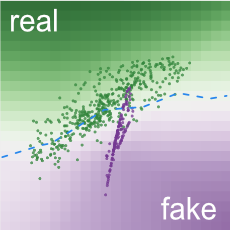
\includegraphics[width=0.4\textwidth]{../Figures/Discriminator.png}
    \caption{The real data points are in green, the fake data points are in purple. The grid color is greener when $D(x)$ is closer to 1, and more purple when closer to 0. Source: \citet{kahng2018gan}}
    \label{fig:discriminator}
\end{figure}

Next, fix the discriminator \(D\) and examine how the choice of \(G\) affects
\(L(D, G)\). Note that the optimal discriminator is \(D(x_i) =
\frac{p_r(x_i)}{p_r(x_i) + p_g(x_i)}\). The optimal generator in this case is
\(G(z) \sim p_r(x)\), which renders the oracle \(D\) equivalent to the ignorant
\(D\)\footnote{Here, \(G\) is essentially saying to \(D\): "I heard you've
    learned something and are no longer an ignorant young kid, but an oracle? Let
    me fool you again."}. If both the discriminator and the generator are at their
optimal states, the loss function evaluates to \(-2\log 2\).

\subsection{Algorithm} \label{subsec:algorithm}

For ease of exposition, we first assume that $G(z;\theta)$ and $D(x;\lambda)$
are parametrized by $\theta$ and $\lambda$, respectively. We summarize it in an
oversimplified way \footnote{Refer to this paper \citet{kaji2023adversarial} or
    the original one \citet{goodfellow2014generative} for the detailed algorithm in
    pseudocode} as follows: One may resort to Figure~\ref{fig:algorithm} for a
visual representation of the algorithm.
\begin{enumerate}
    \item Initialize $\theta^0$ and $\lambda^0$.
    \item While $\theta^k$ has not converged:
          \begin{enumerate}
              \item Generate $x_g$ from $G(z;\theta^k)$.
              \item Train $D(x;\lambda)$ till convergence with $\{x_r\}$ and $\{x^k_g\}$. Update
                    $\lambda^{k+1}$.
              \item Compute the $L(D_{\lambda^{k+1}},G_{\theta^k})$.
              \item Minimize $L(D_{\lambda^{k+1}},G_{\theta^k})$ with respect to $\theta$. Update
                    $\theta^{k+1}$.
          \end{enumerate}
\end{enumerate}

\begin{figure}[!htbp]
    \centering
    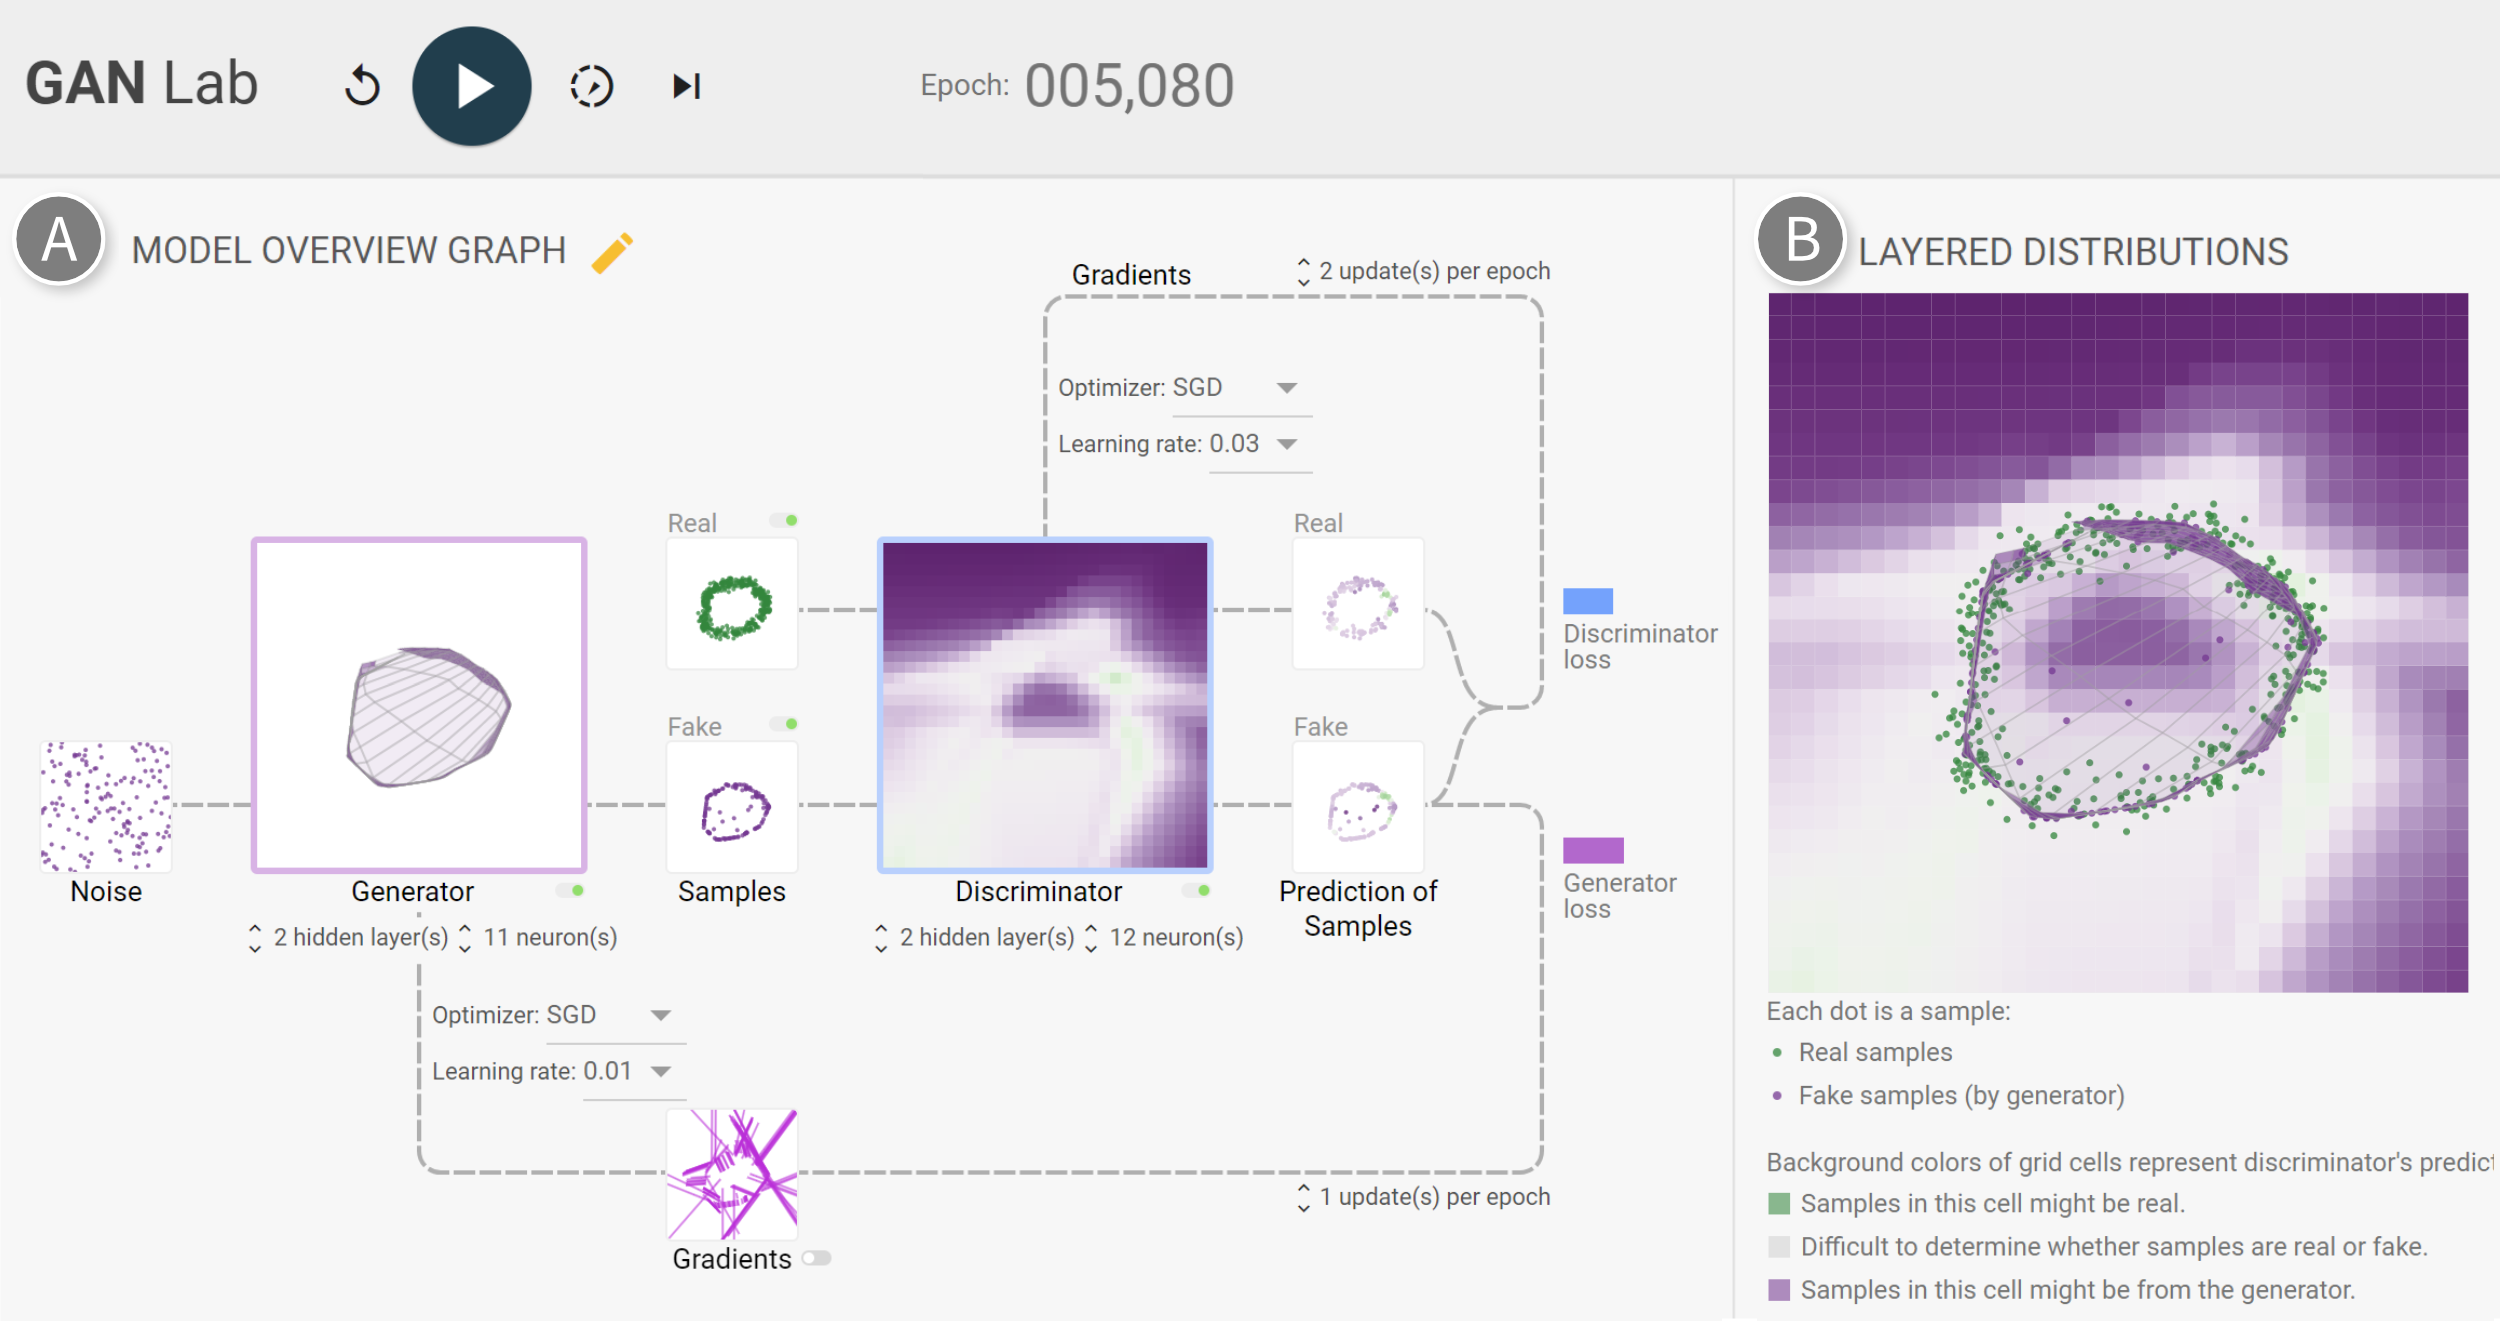
\includegraphics[width=0.8\textwidth]{../Figures/Algorithm.png}
    \caption{The upper-right loop represents the training of $D$ in the step 2.b while the bottom loop represents the training of $G$ in step 2. Source: \citet{kahng2018gan}}
    \label{fig:algorithm}
\end{figure}

When training \(G\), if the true distribution \(p_r\) is parametric (e.g., a
logistic distribution parameterized by location and scale), the training of
\(G\) reduces to estimating the true parameter \(\theta_0\) that characterizes
\(p_r\). If our structural model includes parameters \(\theta\) with the true
value \(\theta_0\) corresponding to the one that generates the observed data,
the generator is trained as an estimator for \(\theta_0\). In the following
section, we denote this adversarial generator estimator as AdE. One may notice
that if the focus is on the generator, the discriminator can be regarded as a
nuisance intermediate step. However, despite being labeled as a nuisance, the
discriminator plays a crucial role in determining the performance of AdE,
including its convergence rate, asymptotic distribution, and efficiency. This
will be further discussed in Section~\ref{sec:performance}.

It is worth noting that in structural parameter estimation, \(G\) is typically
parametric, whereas in the original GAN framework, \(G\) is often implemented
using a neural network. This distinction arises from the different objectives
of the tasks. If the goal is to generate data that mimics the true data, a
neural network is a better choice than a restrictive parametric assumption.
However, if the goal is to estimate the distribution of the true data (rather
than generating new data), the parametric assumption provides interpretable
parameters that are meaningful in an economic context.

The next section~\ref{sec:related_applications} will discuss two applications
of GANs in economics and finance, both of which share the objective of
generating new data.

\section{Related Applications} \label{sec:related_applications}

\subsection{GANs in Economics}
The first paper to apply Wasserstein Generative Adversarial Networks (WGANs) in
economics is \citet{athey2024using}. Unlike traditional GANs, which aim to
generate images that can fool human perception, the authors propose using GANs
to generate synthetic samples that resemble data collected from costly
experiments. For example, consider a program that use conditional subsidy to
encourage school enrollment. The experiment provides researchers with a single
real sample of \(n\) individuals. Researchers can apply various estimators to
this sample to estimate the average treatment effect. However, when
\textbf{evaluating the performance of these estimators}, it is typically
necessary to conduct Monte Carlo simulations using many synthetic samples.
Often, the credibility of such simulations is questioned due to the specific
design choices made in the simulation setup. For instance, an estimator may
appear to perform better solely because of the particular simulation design. To
address this issue, the authors propose using GANs to generate a large of
number of synthetic samples based on which we can evaluate the estimators.

With only one real sample, we can obtain the \textbf{Estimate} and
\textbf{s.e.} columns of Table~\ref{tab:estimator_comparison}. By simulating
2000 replications of the sample using GANs, it is possible to evaluate the
\textbf{RMSE}, \textbf{Bias}, and \textbf{Coverage} of the estimators.

\begin{table}[h!]
    \centering
    \begin{tabular}{|l|c|c|c|c|c|}
        \hline
        \textbf{Method} & \textbf{Estimate} & \textbf{s.e.} & \textbf{RMSE} & \textbf{Bias} & \textbf{Coverage} \\
        \hline
        $\hat{\tau}^1$  & 1.79              & 0.63          & 0.49          & 0.06          & 0.94              \\
        $\hat{\tau}^2$  & 2.12              & 0.88          & 0.58          & 0.00          & 0.96              \\
        $\hat{\tau}^3$  & 1.79              & 0.57          & 0.52          & -0.06         & 0.88              \\
        \hline
    \end{tabular}
    \caption{Comparison of estimators.}
    \label{tab:estimator_comparison}
\end{table}

In addition to the difference in objectives---\citet{athey2024using} focus on
generating data, while \citet{kaji2023adversarial} focus on estimating
parameters---the former uses Wasserstein Generative Adversarial Networks
(WGANs), an improved version of GANs that employs the Wasserstein distance to
measure the difference between the real distribution \(p_r\) and the generated
distribution \(p_g\).

\paragraph{From JS Divergence to Wasserstein Distance}
Recall the GANs objective function in Equation~\ref{eq:gan_objective}. If we
substitute the oracle discriminator \(D_\text{oracle}\), we obtain:
\begin{equation*}
    \begin{split}
        L(G, D_\text{oracle}) & = \int p_r(x) \log \frac{p_r(x)}{p_r(x) + p_g(x)} + p_g(x) \log \frac{p_g(x)}{p_r(x) + p_g(x)} \, dx \\
                              & = 2 L_{JS}(p_r, p_g) - 2 \log 2,
    \end{split}
\end{equation*}
where \(L_{JS}(p_r, p_g)\) is the Jensen-Shannon (JS) divergence between the real and generated distributions. This implies that if the discriminator approximates the oracle, the generator's loss function reduces to the JS divergence between \(p_r\) and \(p_g\). However, the JS divergence has limitations, such as producing non-meaningful divergence values (e.g., \(\infty\)) when the supports of \(p_r\) and \(p_g\) do not overlap. In contrast, the Wasserstein distance provides a meaningful measure of distance between distributions under all circumstances.

To illustrate this, we compare the loss functions for JS divergence and
Wasserstein distance:
\begin{align}
    \min_G \max_D L(G, D) & = \min_G (2 L_{JS}(p_r, p_g) - 2 \log 2), \label{eq:js_loss}                                                                          \\
    \min_G \max_D L(G, D) & = \min_G W(p_r, p_g) \nonumber                                                                                                        \\
                          & = \min_G \max_{w \in W} \left( \mathbb{E}_{x_r \sim p_r}[f_w(x_r)] - \mathbb{E}_{x_g \sim p_g(x)}[f_w(x_g)] \right) \label{eq:w_loss} \\
                          & = \min_G \max_{w \in W} \int \left(p_r(x) - p_g(x)\right) f_w(x) \, dx, \nonumber
\end{align}
where \(\{f_w\}_{w \in W}\) is a family of \(K\)-Lipschitz continuous functions. In this formulation, the discriminator's role is not to classify but to approximate a function \(f_w\) that captures the Wasserstein distance between \(p_r\) and \(p_g\). This explanation closely follows \citet{weng2017gan}, which provides a more detailed explanation of the Wasserstein GANs and its dual formulation.

The algorithm should follow the same structure as in
Figure~\ref{fig:algorithm}, but with modified loss function in
Equation~\eqref{eq:w_loss}.

It would be interesting to see how the Wasserstein GANs perform in the context
of structural estimation. This could be a potential extension of
\citet{kaji2023adversarial}. However, it may be the case that it is not so much
improvment to apply WGAN to economics context since we are not working with
objects like images that often have non-overlapping supports.

\subsection{GANs in Finance}

\section{Performance} \label{sec:performance}

\subsection{Statistical Properties} \label{subsec:statistical_properties}

The adversarial estimator proposed in this paper exhibits several desirable
statistical properties, including consistency, a parametric rate of
convergence, asymptotic normality, and efficiency under correct specification.
These properties are established under a set of assumptions that ensure the
estimator behaves well in both finite and large samples.

\paragraph{Consistency (Theorem 1)} The adversarial estimator \(\hat{\theta}\) converges to \(\theta_0\) if:
\begin{itemize}
    \item The population loss \(M_\theta(D_\theta)\) is uniquely minimized at
          \(\theta_0\),
    \item The classes \(\{\log D_\theta\}\) and \(\{\log(1 - D_\theta) \circ T_\theta\}\)
          satisfy uniform convergence,
    \item \(\mathbb{M}_\theta(\hat{D}_\theta)\) uniformly converges to \(M_\theta(D_\theta)\),
    \item \(\hat{\theta}\) approximately minimizes \(\mathbb{M}_\theta(\hat{D}_\theta)\).
\end{itemize}
\textbf{Result:} \(\hat{\theta} \xrightarrow{p} \theta_0\).

\paragraph{Rate of Convergence (Theorem 2)} Achieves \(\sqrt{n}\)-rate under:
\begin{itemize}
    \item Parametric, smooth structural model (Assumption 1),
    \item \(m/n \to \infty\) (Assumption 2),
    \item Orthogonality of discriminator estimation (Assumption 3),
    \item Quadratic curvature of \(M_\theta(D_\theta)\) (Assumption 4).
\end{itemize}
\textbf{Result:} \(h(\hat{\theta}, \theta_0) = O_p(n^{-1/2})\).

\paragraph{Asymptotic Distribution (Theorem 3)} Under regularity conditions:
\[
    \sqrt{n}(\hat{\theta} - \theta_0) \xrightarrow{d} N\left(0, \frac{1}{4} \bar{I}_{\theta_0}^{-1} V \bar{I}_{\theta_0}^{-1}\right),
\]
where \(V = \lim 4P_{\theta_0}[D_{\theta_0}(1 -
        D_{\theta_0})\dot{\ell}_{\theta_0}\dot{\ell}_{\theta_0}^\top]\).

\paragraph{Efficiency (Corollary 4)} Under correct specification:
\[
    \sqrt{n}(\hat{\theta} - \theta_0) \xrightarrow{d} N(0, I_{\theta_0}^{-1}),
\]
achieving the Cramér-Rao bound when \(m \gg n\).

\subsection{Comparison} \label{subsec:comparison}
\begin{quote}
    The adversarial estimator fills the gap between SMM and MLE.
\end{quote}

There are numerous existing methods for structural estimation. This section
compares the newly proposed adversarial estimator (AdE) with maximum likelihood
estimation (MLE), simulated method of moments (SMM), and simulated maximum
likelihood (SML). The paper claims that AdE does not require a tractable
likelihood or a correctly specified discriminator, nor does it suffer from the
issues associated with an increasing number of moment conditions. To provide a
comprehensive comparison, we include SML as a method for handling intractable
likelihoods. Below, we outline the objective functions of each method.

\paragraph{MLE}
The maximum likelihood estimator minimizes the negative log-likelihood:
\begin{equation*}
    \min_\theta L_\theta = -\frac{1}{n} \sum_{i=1}^n \log p(x_i; \theta),
\end{equation*}
where \(p(x; \theta)\) is the probability density of observing the real data \(x\) under the model parameterized by \(\theta\).

\paragraph{AdE}
The adversarial estimator minimizes the following objective:
\begin{equation*}
    \min_\theta M_\theta(D) = \frac{1}{n} \sum_{i=1}^n \log D(x_i) + \frac{1}{m} \sum_{j=1}^m \log \left(1 - D(G_\theta(z_j))\right),
\end{equation*}
where \(D(x; \lambda)\) is the discriminator's probability that \(x\) is real, and \(G_\theta(z)\) is the generator mapping noise \(z\) to synthetic data. Although the objective functions of MLE and AdE appear similar, \(p(x; \theta)\) and \(D(x; \lambda)\) represent fundamentally different quantities: the former is the likelihood of the data, while the latter is a discriminator estimating the probability that \(x\) belongs to the real sample.

\paragraph{SMM}
The simulated method of moments relies on moment conditions of the form
\(\mathbb{E}_X[f(X; \theta)] = \theta\), where \(f(X; \theta)\) is a moment
function. By replacing \(\theta\) with a generator \(G\), we impose the
condition \(\mathbb{E}_Z[G(Z; \theta)] = \theta\). The theoretical moment
condition becomes:
\begin{equation*}
    \mathbb{E}_X\left[f(X; \theta) - \mathbb{E}_Z[G(Z; \theta)]\right] = 0.
\end{equation*}
The SMM objective function is:
\begin{equation*}
    \min_\theta S_\theta = \left\{\frac{1}{n}\sum_{i=1}^n \left[f(X_i) - \frac{1}{m} \sum_{j=1}^m G(Z_j; \theta)\right]\right\}^\top \Omega \left\{\frac{1}{n}\sum_{i=1}^n \left[f(X_i) - \frac{1}{m} \sum_{j=1}^m G(Z_j; \theta)\right]\right\},
\end{equation*}
where \(n\) and \(m\) are the sizes of the real and synthetic datasets, respectively. Consistency of SMM estimator requires $n\to\infty$ while holding $m$ fixed. Unlike AdE, the generator \(G\) in SMM is not an estimator but a function used to construct moment conditions. Finding such a generator \(G\) that satisfies \(\mathbb{E}_Z[G(Z; \theta)] = \theta\) can be challenging.

\paragraph{SML}
Simulated maximum likelihood (SML) addresses intractable likelihoods by
approximating the likelihood function. Suppose the likelihood \(p(x; \theta)\)
is not analytically computable. We introduce a function \(G(x, z; \theta)\)
such that \(\mathbb{E}_z[G(x, z; \theta)] = p(x; \theta)\). Or we consider a
more general form with both $y_i$ and $x_i$. Since \(p(y_i \mid x_i; \theta)\)
is intractable, we simulate \(m\) draws \(z_{ir}\) for each \((x_i, y_i)\) and
approximate the likelihood as:
\begin{equation*}
    L_s(\theta) = \prod_{i=1}^n \left[\frac{1}{m} \sum_{r=1}^m G(y_i \mid x_i, z_{ir}; \theta)\right].
\end{equation*}
In log form, the SML objective becomes:
\begin{equation*}
    \ell_s(\theta) = \sum_{i=1}^n \log \left[\frac{1}{m} \sum_{r=1}^m G(y_i \mid x_i, z_{ir}; \theta)\right].
\end{equation*}
Under regularity conditions, the SML estimator \(\hat{\theta}\) is consistent as \(m \to \infty\) and \(n \to \infty\).

\subsection{Discussion} \label{subsec:discussion}

In the previous subsection, we outlined the objective functions for MLE, AdE,
SMM, and SML. Focusing on the three simulation-based methods—AdE, SMM, and
SML—we observe interesting differences in their requirements for sample size
\(n\) and simulation size \(m\) for convergence. Specifically:

\begin{itemize}
    \item \textbf{SMM} requires \(n \to \infty\) while holding \(m\) fixed to achieve a parametric rate of convergence.
    \item \textbf{SML} requires both \(n \to \infty\) and \(m \to \infty\) to achieve a parametric rate.
    \item \textbf{AdE} requires uniform convergence of \(\mathbb{M}_\theta(\hat{D}_\theta)\) to \(M_\theta(D_\theta)\) and, to achieve the parametric rate, \(m/n \to \infty\).
\end{itemize}

Secondly, in terms of asymptotic distribution, AdE is more ambiguous because
notice that the distribution is derived assuming that the there exists a
likelihood and is twice differentiable. This is somewhat restrictive statement
because one of the reason we promote AdE is that it performs well when the
likelihood is intractable. In this sense, inference on the estimates coming
from AdE is less theoretically gounded than the other methods. The paper
presents standard error of the AdE estimates using bootstrap method (500
replications with $\set{X_i}_i^n$ and $\set{Z_j}_j^n$), while stating that this
is not theoretically proven. This is one of the drawback of AdE.

Thirdly, to see the efficiency of the AdE, we take the figures in the paper.
Figure~\ref{fig:MLE_AdE_NN} shows that if the model is correctly specified,
which means that if the true distribution is $\text{Logistic}~(0,1)$, the
specified structural model is $\text{Logistic}~(\theta,1)$. The AdE with neural
network discriminator works as good as MLE. When the model is misspecified, the
pseudo-likelihood and the oracle loss differs by a lot. Note that the oracle
loss is when we take the discriminator to be
$\frac{p'_{r,\theta}}{p'_{r,\theta}+p_g}$. Since we specify the form of $p'_r$
wrongly, the oracle $D$ is not the same as the one under the correct model of
the real distribution $\frac{p_{r,\theta}}{p_{r,\theta}+p_g}$. The paper claims
that the performance is close to that of qMLE as shown in
Figure~\ref{fig:QMLE_AdE}.
\begin{figure}
    \centering
    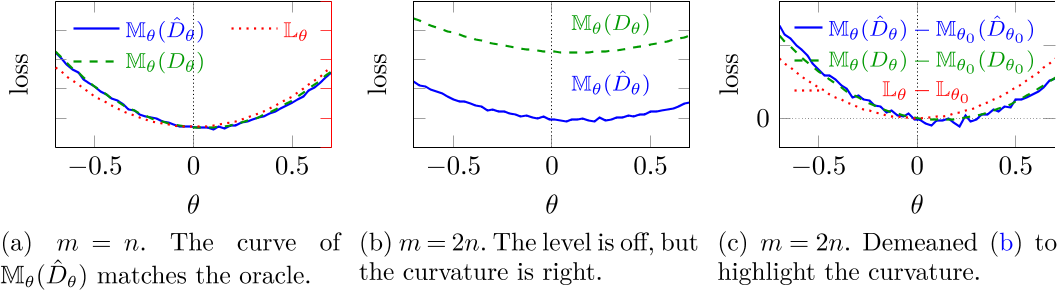
\includegraphics[width=0.8\textwidth]{../Figures/MLE_AdE_NN.png}
    \caption{The objective function of MLE and AdE (with neural network discriminator). Source: \citet{kaji2023adversarial}}
    \label{fig:MLE_AdE_NN}
\end{figure}

\begin{figure}
    \centering
    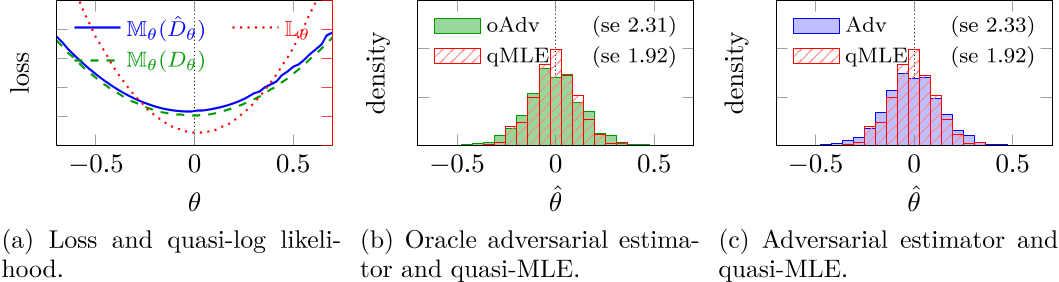
\includegraphics[width=0.8\textwidth]{../Figures/QMLE_AdE.png}
    \caption{The objective function of QMLE and AdE. Source: \citet{kaji2023adversarial}}
    \label{fig:QMLE_AdE}
\end{figure}

When it comes to comparing with SMM, the paper compare optimal weighted SMM
with AdE in such a way that there is increasing number of constraints. For SMM,
there are $d=3,7,11$ number of moment conditions to match while in AdE, the
discriminator has has $d=3,7,11$ parameters $\lambda$. More concrete, SMM's
mopment takes the form $\mathbb{E}_{X}(f(X|\theta)) = \theta \quad
    f(X|\theta)\in \mathbb{R}^d$ which is number of $d$ order condition. AdE's
discriminator takes the form $D(x,x^2,\ldots,x^d;\lambda_0,\ldots,\lambda_d)$
Figure~\ref{fig:SMM_AdE} only shows the actual likelihood and oracle loss and
the estimated loss of AdE. Only the estimated loss of AdE is changing as the
number of input to the discriminator increases. It seems a bit unnatural to not
show the objective function of SMM here for comparison. Moreover, varying the
flexibility $d$ of the discriminator does not appeal to me if what is
recommended is using a NN discriminator to approximate the oracle loss.

\begin{figure}
    \centering
    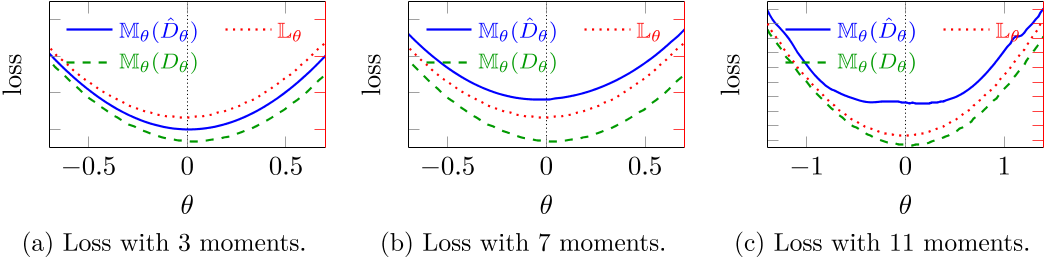
\includegraphics[width=0.8\textwidth]{../Figures/SMM_AdE.png}
    \caption{The objective function AdE with $d=3,7,11$ input to the discriminator. Source: \citet{kaji2023adversarial}}
    \label{fig:SMM_AdE}
\end{figure}

Lastly, One might question the necessity of AdE given the existence of SMM and
SML. However, AdE offers a distinct advantage in scenarios where constructing a
simulator function \(G\) is challenging. Specifically, SMM requires a function
\(G\) such that \(\mathbb{E}_Z[G(Z; \theta)] = \theta\), and SML requires \(G\)
to satisfy \(\mathbb{E}_z[G(x, z; \theta)] = p(x; \theta)\). In practice,
finding such functions can be non-trivial or even infeasible. AdE circumvents
this issue by leveraging a discriminator to guide the generator, eliminating
the need for an explicit simulator function. This flexibility makes AdE
particularly appealing for complex structural models.

That said, AdE is not without its challenges. Computational concerns arise due
to the iterative nature of adversarial training, which involves alternating
updates between the generator and discriminator. This process can be
computationally intensive and sensitive to hyperparameter choices, such as the
learning rate and network architecture. Despite these challenges, AdE
represents a powerful and flexible alternative to traditional simulation-based
methods, especially in settings where constructing a simulator function is
impractical.

To conclude, the adversarial estimator offers a promising alternative to
structural estimation with desirable propoerties. If we can leverage the
computation power in training the estimator, especially the training of the
discriminator, we can expect the estimator to perform well in practice.
Therefore, future work to promote AdE should focus on developing well-optimized
easy to use training algorithms for economics researchers as well as devloping
inference for the AdE esetiamtes

% - Why use GANs?
% - Why is it superior to SMM and SML or MLE?

% - Computation overhead?
% - Is there a package that one can utilize to implement the method?

% - Add some performance comparison figure from the paper 
% - Asymptotic distribution: intractible likelihood. then variance of the estimatior is difficult to get. Bootsrap is not theoretically proven.

% To promote the method, thus inference may be difficult to get. next step: inference and computation.

\pagebreak
\newpage
\bibliography{ref.bib}

\end{document}